\section{Natural Language Processing}\label{sec:nlp}
%**************************************************************

The field of \gls{nlp}, also known as computational linguistics, is a branch of Artificial Intelligence focused on the technology of processing language.
It encompasses a variety of topics, which involves the engineering of computational models and
processes to solve practical problems in understanding and generating human
languages. These solutions are used to build useful software.

The linguistics computational has two
branches---computational linguistics and theoretical linguistics. The computational
linguistics has been concerned with developing algorithms for handling a useful
range of natural language as input. While the theoretical linguistics has focused
primarily on one aspect of language performance, grammatical competence---how
people accept some sentences as correctly following grammatical rules and others as ungrammatical. They are concerned with language universals—principals of
grammar which apply to all natural languages \cite{Cole:1996}.

Computational linguistics is concerned with the study of natural language analysis
and language generation. Further, the language analysis is divided into two domains,
namely sentence analysis, and discourse and dialogue structure. Much more is known
about the processing of individual sentences than about the determination of discourse
structure. Any analysis of discourse structure requires a prerequisite as an analysis of
the meaning of individual sentences. However, it is a fact that for many applications,
thorough analysis of discourse is not mandatory, and the sentences can be understood
without that \cite{grishman_computational_1986}.

The sentence analysis is further divided into syntax analysis and semantic analysis.
The overall objective of sentence analysis is to determine what a sentence “means”.
In practice, this involves translating the natural language input into a language with
simple semantics, for example, formal logic, or into a database command language.
In most systems, the first stage is syntax analysis. Figure \ref*{fig:nlp_components} shows the relations
among different components of NLP \cite{Chowdhary2020}.

\begin{figure}[H]
    \centering
    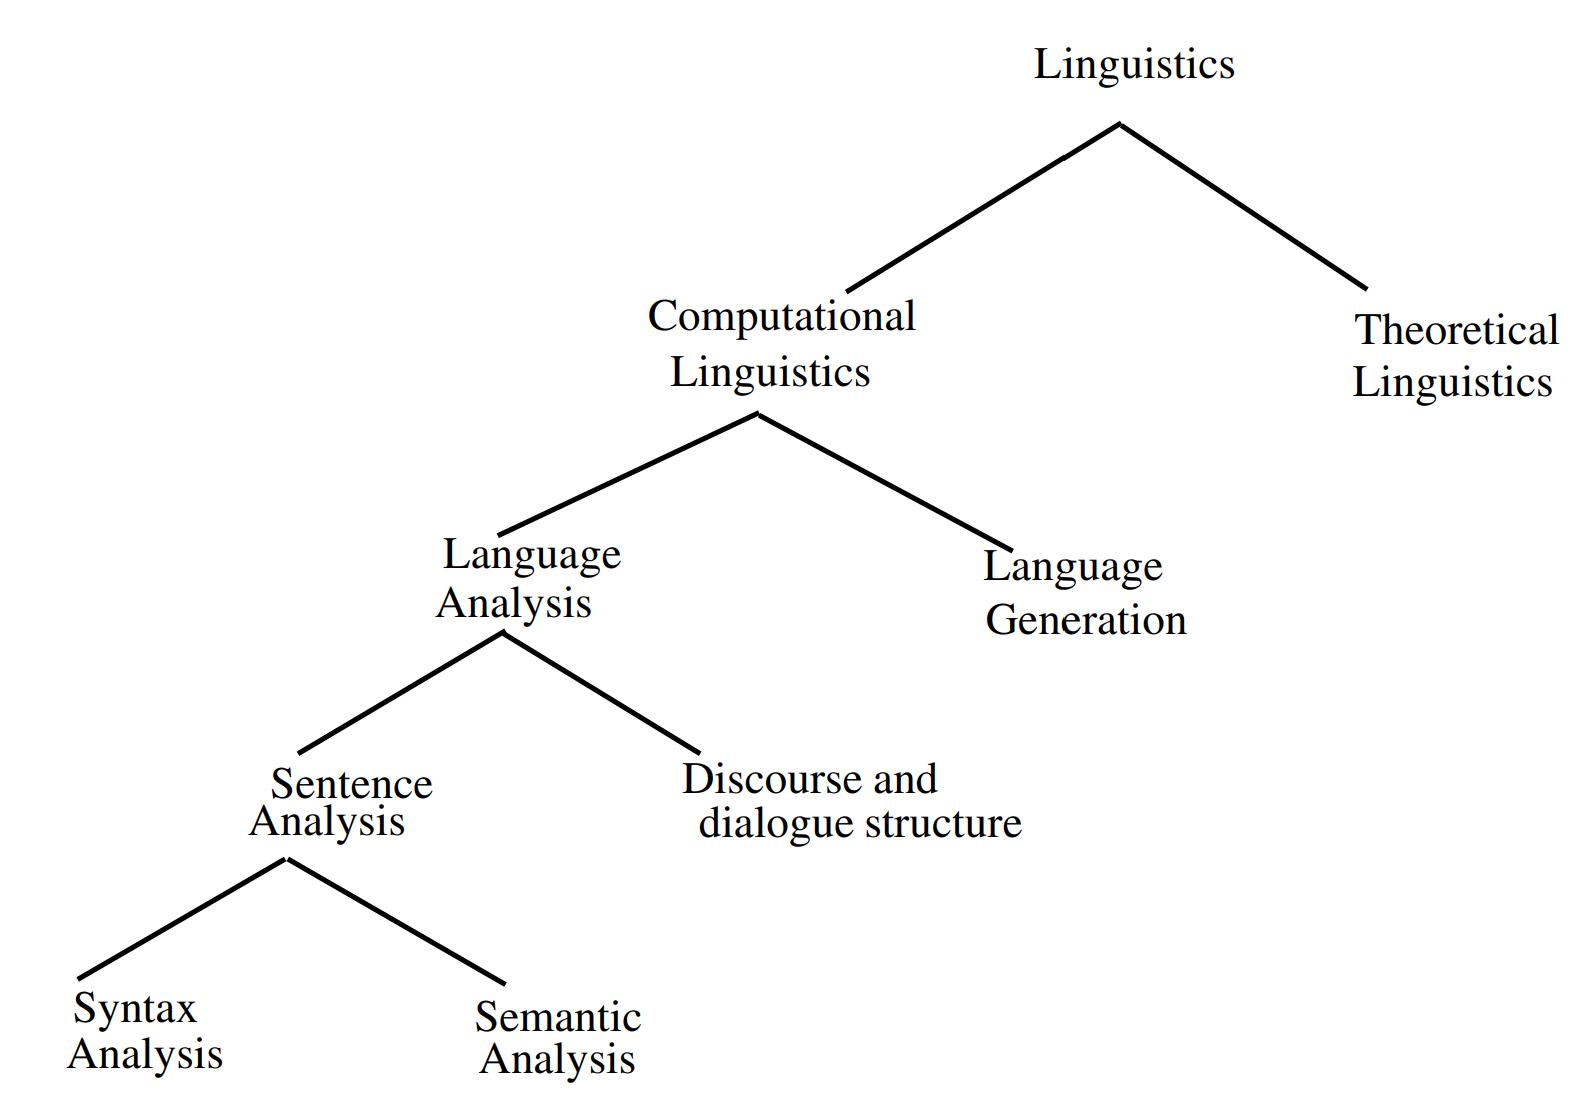
\includegraphics[width=0.8\textwidth]{images/2_1_nlp_components.png}
    \caption{Components of NLP}\label{fig:nlp_components}
\end{figure}
    

Some of the common applications of NLP are: Classification of text into categories, Index and search large texts, Automatic translation, Information extraction,
Automatic summarization, Question answering, Knowledge acquisition, and Text
generations/dialogues.
Some of those tasks are discussed in sections \ref{subsec:text-classification}, \ref{subsec:sentiment-analysis}, \ref{subsec:nli}, \ref{subsec:seq2seq}.

%**************************************************************

\subsection{Lexicon}\label{subsec:lexicon}
Dictionaries are special texts whose subject matter is
a language, or a pair of languages in the case of a
bilingual dictionary. The purpose of dictionaries is to
provide a wide range of information about words---
etymology, pronunciation, stress, morphology, syntax, register---to give definitions of senses of words,
and, in so doing, to supply knowledge not just about
language, but about the world itself.

The term “dictionary” is typically related to printed wordbook for human readers. 
Instead “\gls{lexicon}” will refer to the component of
a NLP system that contains information (semantic,
grammatical) about individual word strings \cite{Guthrie_ComACM96}.

A lexicon which provides an effective combination of traditional
lexicographic information and modern computing is called WordNet \cite{miller1995wordnet}.
It is an online lexical database designed for use under program control. English nouns, verbs,
adjectives, and adverbs are organized into sets of synonyms, each representing
a lexicalized concept. WordNet contains more than 118,000 different word
forms and more than 90,000 different word senses. Approximately 40\% of
the words in WordNet have one or more synonyms.

The cognitive synonyms which are called synsets are presented in the database with lexical and semantic relations. 
WordNet includes the following semantic relations:
\begin{itemize}
    \item \textbf{Hypernymy}: A hypernym is a word that is more general than the word in question. For example, the hypernym of “dog” is “canine”.
    \item \textbf{Hyponymy}: A hyponym is a word that is more specific than the word in question. For example, the hyponym of “dog” is “poodle”.
    \item \textbf{Synonymy}: A synonym is a word that has the same meaning as the word in question. For example, the synonym of “good” is “well”.
    \item \textbf{Antonymy}: An antonym is a word that has the opposite meaning of the word in question. For example, the antonym of “good” is “bad”.
\end{itemize}

%**************************************************************

\subsection{Word Embeddings}\label{subsec:word-embeddings}
The way machine learning models process data is different from how humans do. 
For example, we can easily understand the text “I saw a cat”, but our models can not --- they need vectors of features. 
Such vectors, called \glsplural{word embedding}, are representations of words which can be fed into a model.


\subsubsection{Bag of words}\label{subsubsec:bag-of-words}
A common approach to represent a text document is to use a column vector of word counts.
This embedding is often called a \gls{bag-of-words}, because it includes only information about the count of each word, and not the order in which the words appear.

The bag-of-words representation ignores grammar, sentence boundaries, paragraphs — everything but the words. Yet the bag of words model is surprisingly effective for text classification.
In the example in the Figure \ref{fig:bag_of_words}, instead of representing the word order in all the phrases like “I love this movie” and “I would recommend it”, we simply note that the word I occurred 5 times in the entire excerpt, the word it 6 times, the words love, recommend, and movie once, and so on \cite{Jurafsky2009}.

\begin{figure}[H]
    \centering
    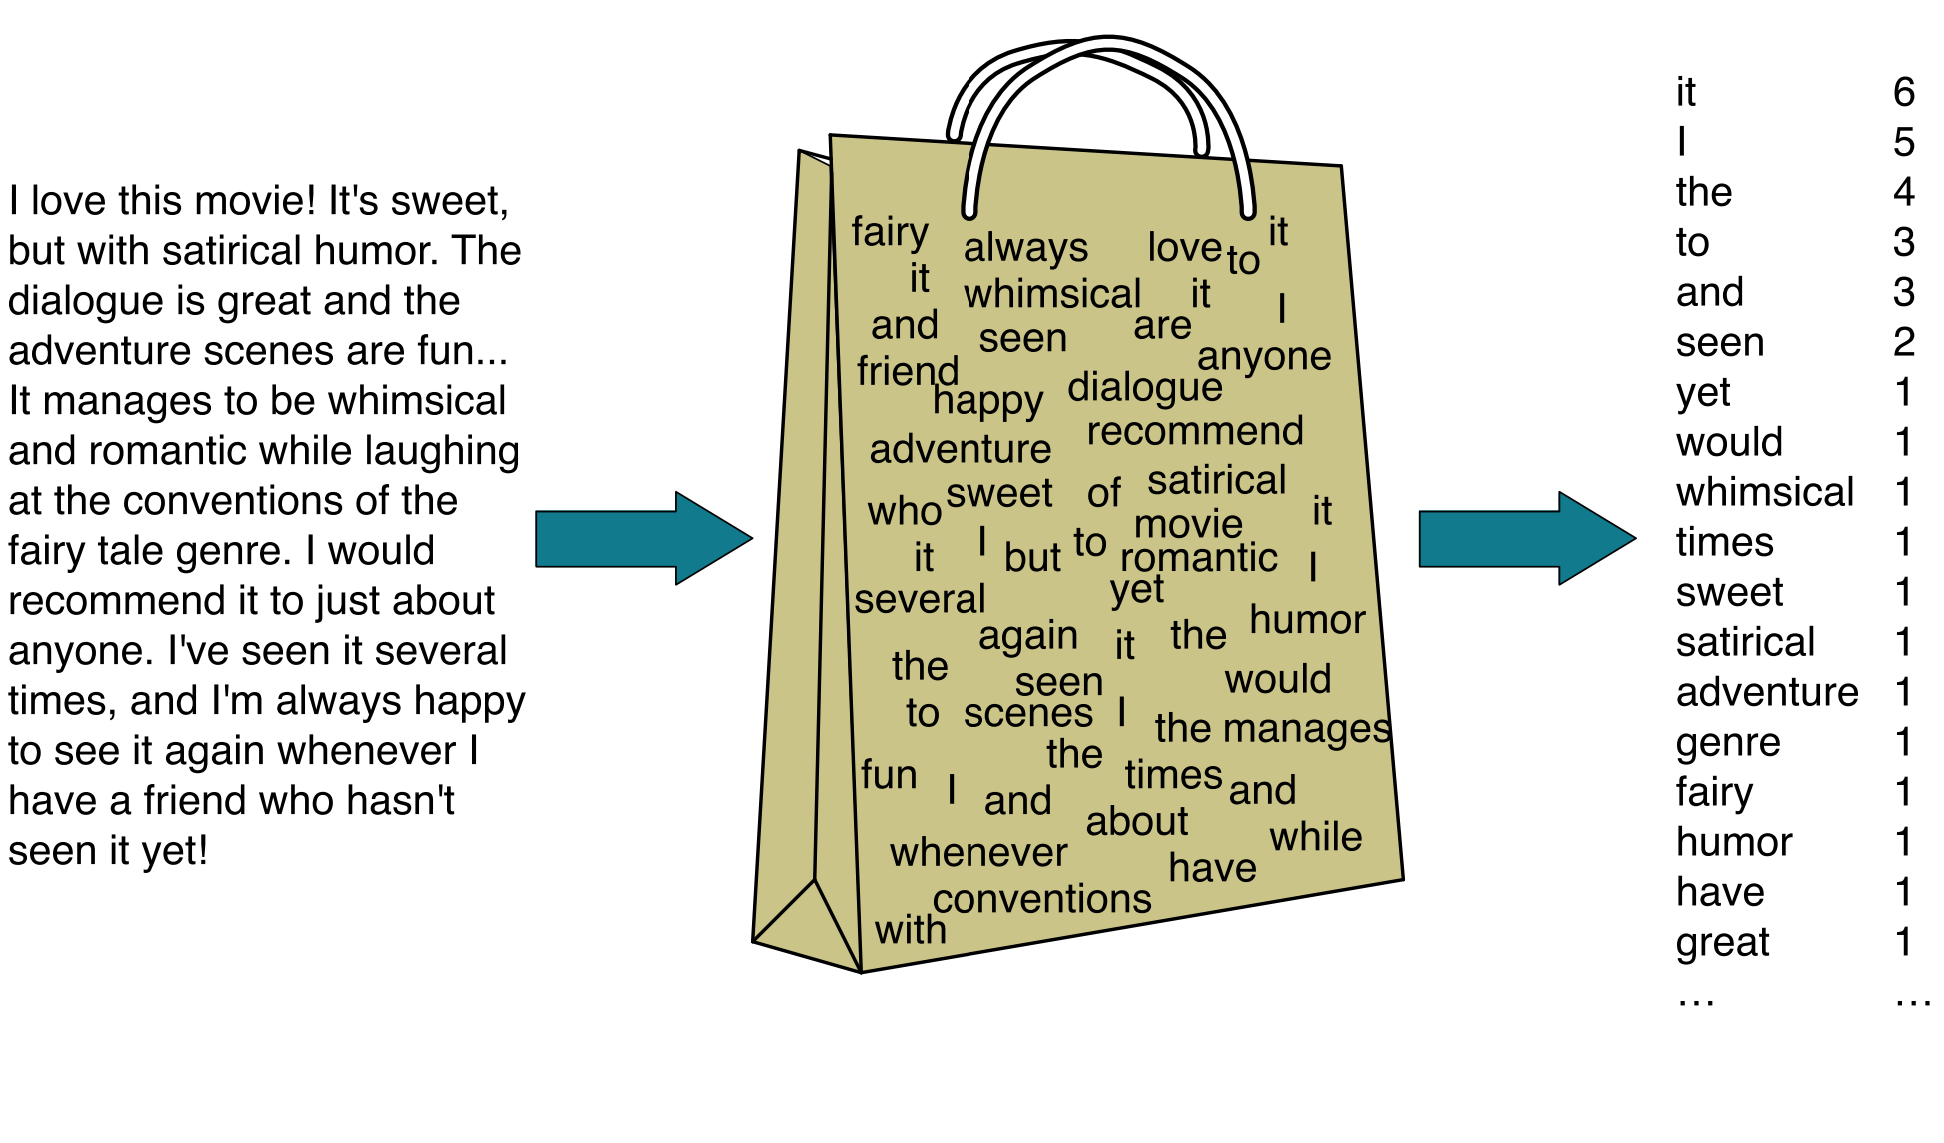
\includegraphics[width=0.8\textwidth]{images/2_1_bag_of_words.png}
    \caption{Bag-of-words representation of a a movie review, where only the frequency of each word is considered.}\label{fig:bag_of_words}
\end{figure}


\subsubsection{Dense embeddings}\label{subsubsec:static-embeddings}
Bag-of-words embeddings are sparse and long vector with dimensions corresponding to words in the vocabulary or documents in a collection.
A more powerful word representation is a dense vector, where instead of mostly-zero counts, the values will be real-valued numbers that can be negative.
It turns out that dense vectors work better in every NLP task than sparse vectors.

Bengio et al. \cite{conf/nips/BengioDV00} presented a model which learned word representations using distributed
representation. Authors presented a neural model which obtains word representations as to
the product while training \gls{language-model}.
The popularity of word representation methods are due to two famous models, Word2Vec
\cite{mikolov2013efficient} and GloVe \cite{pennington2014glove}.

\subsubsection{Contextual embeddings}\label{subsubsec:contextual-embeddings}
To address the issue of polysemous and the context-dependent nature of words, we need
distinguish the semantics of words in different contexts.

Contextualised word embeddings are variable vector that are dependent on the context in which the word is used.
So, representations of a given word are multiple and are
directly computed from their context. The context of a
word is usually composed by the words surrounding it.

These contextualized representations are set to the hidden states of a deep neural model, which is trained as a language model.
By running the language model, we obtain contextualized word representations, which can then be used as the base layer in a supervised neural network for any task. This approach yields significant gains over pretrained word embeddings on several tasks, presumably because the contextualized embeddings use unlabeled data to learn how to integrate linguistic context into the base layer of the supervised neural network.


%**************************************************************

\subsection{Masked Language Models}\label{subsec:masked-language-models}
A \acrfull{mlm} is a pre-training technique whichc first masks out some tokens from the
input sentences and then trains the model to predict the masked
tokens by the rest of the tokens. A special \texttt{[MASK]} token is used to replace some words randomly into the original text.

Masked Language Modelling is usually solved as classification problem. We feed the masked
sequences to a neural encoder whose output vectors are further fed into a softmax classifier to predict the masked token.

The most popular MLM is \acrshort{bert} \cite{devlin2018bert}, which is a bidirectional encoder representation from a particular deep learning architecture called \gls{transformer} \cite{vaswani2017attention}. 
It uses self-supervised training on the masked language modeling and next sentence prediction tasks to learn/produce contextual representations of words.

Concurrently, there are multiple research proposing different enhanced versions of MLM to further improve on BERT. Instead
of static masking, RoBERTa \cite{liu2019roberta} improves BERT by dynamic masking.
While other models aim to optimize BERT's performance, DistilBERT has a different goal. Its target is to reduce the large size and enhance the speed of BERT while still keeping as much strength as possible.
DistilBERT \cite{sanh2019distilbert} reduces the size of $BERT_{BASE}$ by 40\%, enhances the speed by 60\% while retaining 97\% of its capabilities.
ALBERT \cite{lan2019albert} also reduces the model size of BERT, it does not have to trade-off the performance. Compared to DistilBERT, which uses BERT as the teacher for its distillation process, ALBERT is trained from scratch (just like BERT).

%**************************************************************
\subsection{Text classification}\label{subsec:text-classification}

Classification lies at the heart of both human and machine intelligence. Deciding what letter, word, or image has been presented to our senses, recognizing faces or voices, sorting mail, assigning grades to homeworks; these are all examples of assigning a category to an input.
In this section we introduce text classification, the task of assigning a label or category to an entire text or document.

Given a text document, assign it a discrete label $y \in Y$, where $Y$ is the set of possible labels. 
Text classification has many applications, from spam filtering to the analysis of electronic health records, or the categorization of news articles.

Classification is essential for tasks below the level of the document as well.
An example of this is period disambiguation (deciding if a period is the end of a sentence or part of a word), or word tokenization (deciding if a character should be a word boundary). Even language modeling can be viewed as classification: each word can be thought of as a class, and so predicting the next word is classifying the context-so-far into a class for each next word. A part-of-speech tagger classifies each occurrence of a word in a sentence as, e.g., a noun or a verb.

The goal of classification is to take a single observation, extract some useful features, and thereby classify the observation into one of a set of discrete classes.

One method for classifying text is to use handwritten rules. There are many areas of language processing where handwritten rule-based classifiers constitute a state-ofthe-art system, or at least part of it. Rules can be fragile, however, as situations or data change over time, and for
some tasks humans aren't necessarily good at coming up with the rules. Most cases of classification in language processing are instead done via supervised machine learning, where an algorithm learn how to map from an observation to a correct output \cite{Jurafsky2009}.

Many kinds of machine learning algorithms are used to build classifiers.
Formerly, statistical and machine learning approaches, such as naïve Bayes, k-nearest neighbors, hidden Markov models, conditional random fields (CRFs), decision trees, random forests, and support vector machines, were widely used to design classifiers. 
However, during the past several years, there has been a wholesale transformation, and these approaches have been entirely replaced, or at least enhanced, by neural network models \cite{surveyNlpDeepLearning}. 

%**************************************************************
\subsection{Sentiment analysis}\label{subsec:sentiment-analysis}
A popular application of text classification is sentiment analysis, the extraction of sentiment, the positive or negative orientation that a writer expresses toward some object. A review of a movie, book, or product on the web expresses the author's sentiment toward the product, while an editorial or political text expresses sentiment toward a candidate or political action. Extracting consumer or public sentiment is thus relevant for fields from marketing to politics. \cite{Jurafsky2009}

The simplest version of sentiment analysis is a binary classification task, and
the words of the review provide excellent cues. Consider, for example, the following phrases extracted from positive and negative reviews of movies and restaurants. Words like great, richly, awesome, and pathetic, and awful and ridiculously are very informative cues:

\emph{$+$ ...zany characters and richly applied satire, and some great plot twists}
\par
\emph{$-$ It was pathetic. The worst part about it was the boxing scenes...}
\par
\emph{$+$ ...awesome caramel sauce and sweet toasty almonds. I love this place!}
\par
\emph{$-$ ...awful pizza and ridiculously overpriced...} 

The area of sentiment analysis it is becoming increasingly popular and utilizing deep learning. Applications are varied, including product research, futures prediction, social media analysis, and classification of spam \cite{ZhengWG18}. 
Good results were obtained using an ensemble, including both \acrshortpl{lstm} and \acrshortpl{cnn} \cite{Cliche17}.
But the current trend in state-of-the-art models in all application areas is to use pretrained stacks of transformer units in some configuration, whether in encoder-decoder configurations or just as encoders.

%**************************************************************

\subsection{Natural language inference}\label{subsec:nli}

The task of \acrfull{nli}, also
known as recognizing textual entailment,
asks a system to evaluate the relationships between
the truth-conditional meanings of two sentences
or, in other words, decide whether one sentence
follows from another.
The relationship can be entailment, contradiction, or neutral.

Specifically, natural language inference (NLI)
is concerned with determining whether a natural language hypothesis \emph{h} can be inferred from a
premise \emph{p}, as depicted in the following example
from \cite{Manning2009NaturalLI}, where the hypothesis is
regarded to be entailed from the premise.

\emph{p: Several airlines polled saw costs grow more than
expected, even after adjusting}
\par
\emph{$\quad$ for inflation.}
\par
\emph{h: Some of the companies in the poll reported cost
increases.}


%**************************************************************

\subsection[Seq2Seq]{Sequence-to-Sequence models}\label{subsec:seq2seq}

All the tasks we have discussed so far are classification-based, where the input is a text and the output is a label. However, there are many tasks where the input and output are both sequences of tokens. 
For example, machine translation, summarization, and question answering are all tasks where we want to generate a sequence in human-like language as output.

A \acrfull{seq2seq} model is  is a special class of \acrfull{rnn} architectures  that can be used to solve these tasks.

In the general case, input sequences and output sequences have different lengths (e.g. machine translation) and the entire input sequence is required in order to start predicting the target. This requires a more advanced setup:
\begin{itemize}
    \item An \emph{encoder} processes the input sequence and returns its own internal state. This vector is called the context vector.
    \item A \emph{decoder} is a neural network that takes the context vector as input and outputs a sequence of tokens. It is trained to predict the next characters of the target sequence, given previous characters of the target sequence. 
\end{itemize}


An example of this architecture is shown in Figure \ref{fig:seq2seq}.
\begin{figure}[ht]
    \centering
    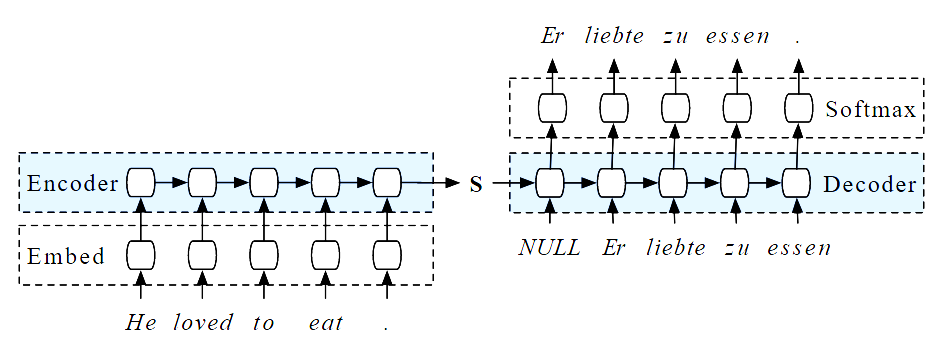
\includegraphics[width=0.8\linewidth]{images/2_1_seq2seq.png}
    \caption{An example of a sequence-to-sequence model for machine translation.}
    \label{fig:seq2seq}
\end{figure}



%**************************************************************
